\chapter{Full Requirements}
\label{sec:reqs}
\section{Framework}
\section{Fully Functional Tool}
\section{Client and GUI}
\cleardoublepage
\begingroup
\advance\textwidth\pdfpagewidth
\hsize=\textwidth\linewidth=\hsize\columnwidth=\hsize
\pdfpagewidth=2\pdfpagewidth

\chapter{Architechture Diagram}
\label{sec:archdesign}
\centering
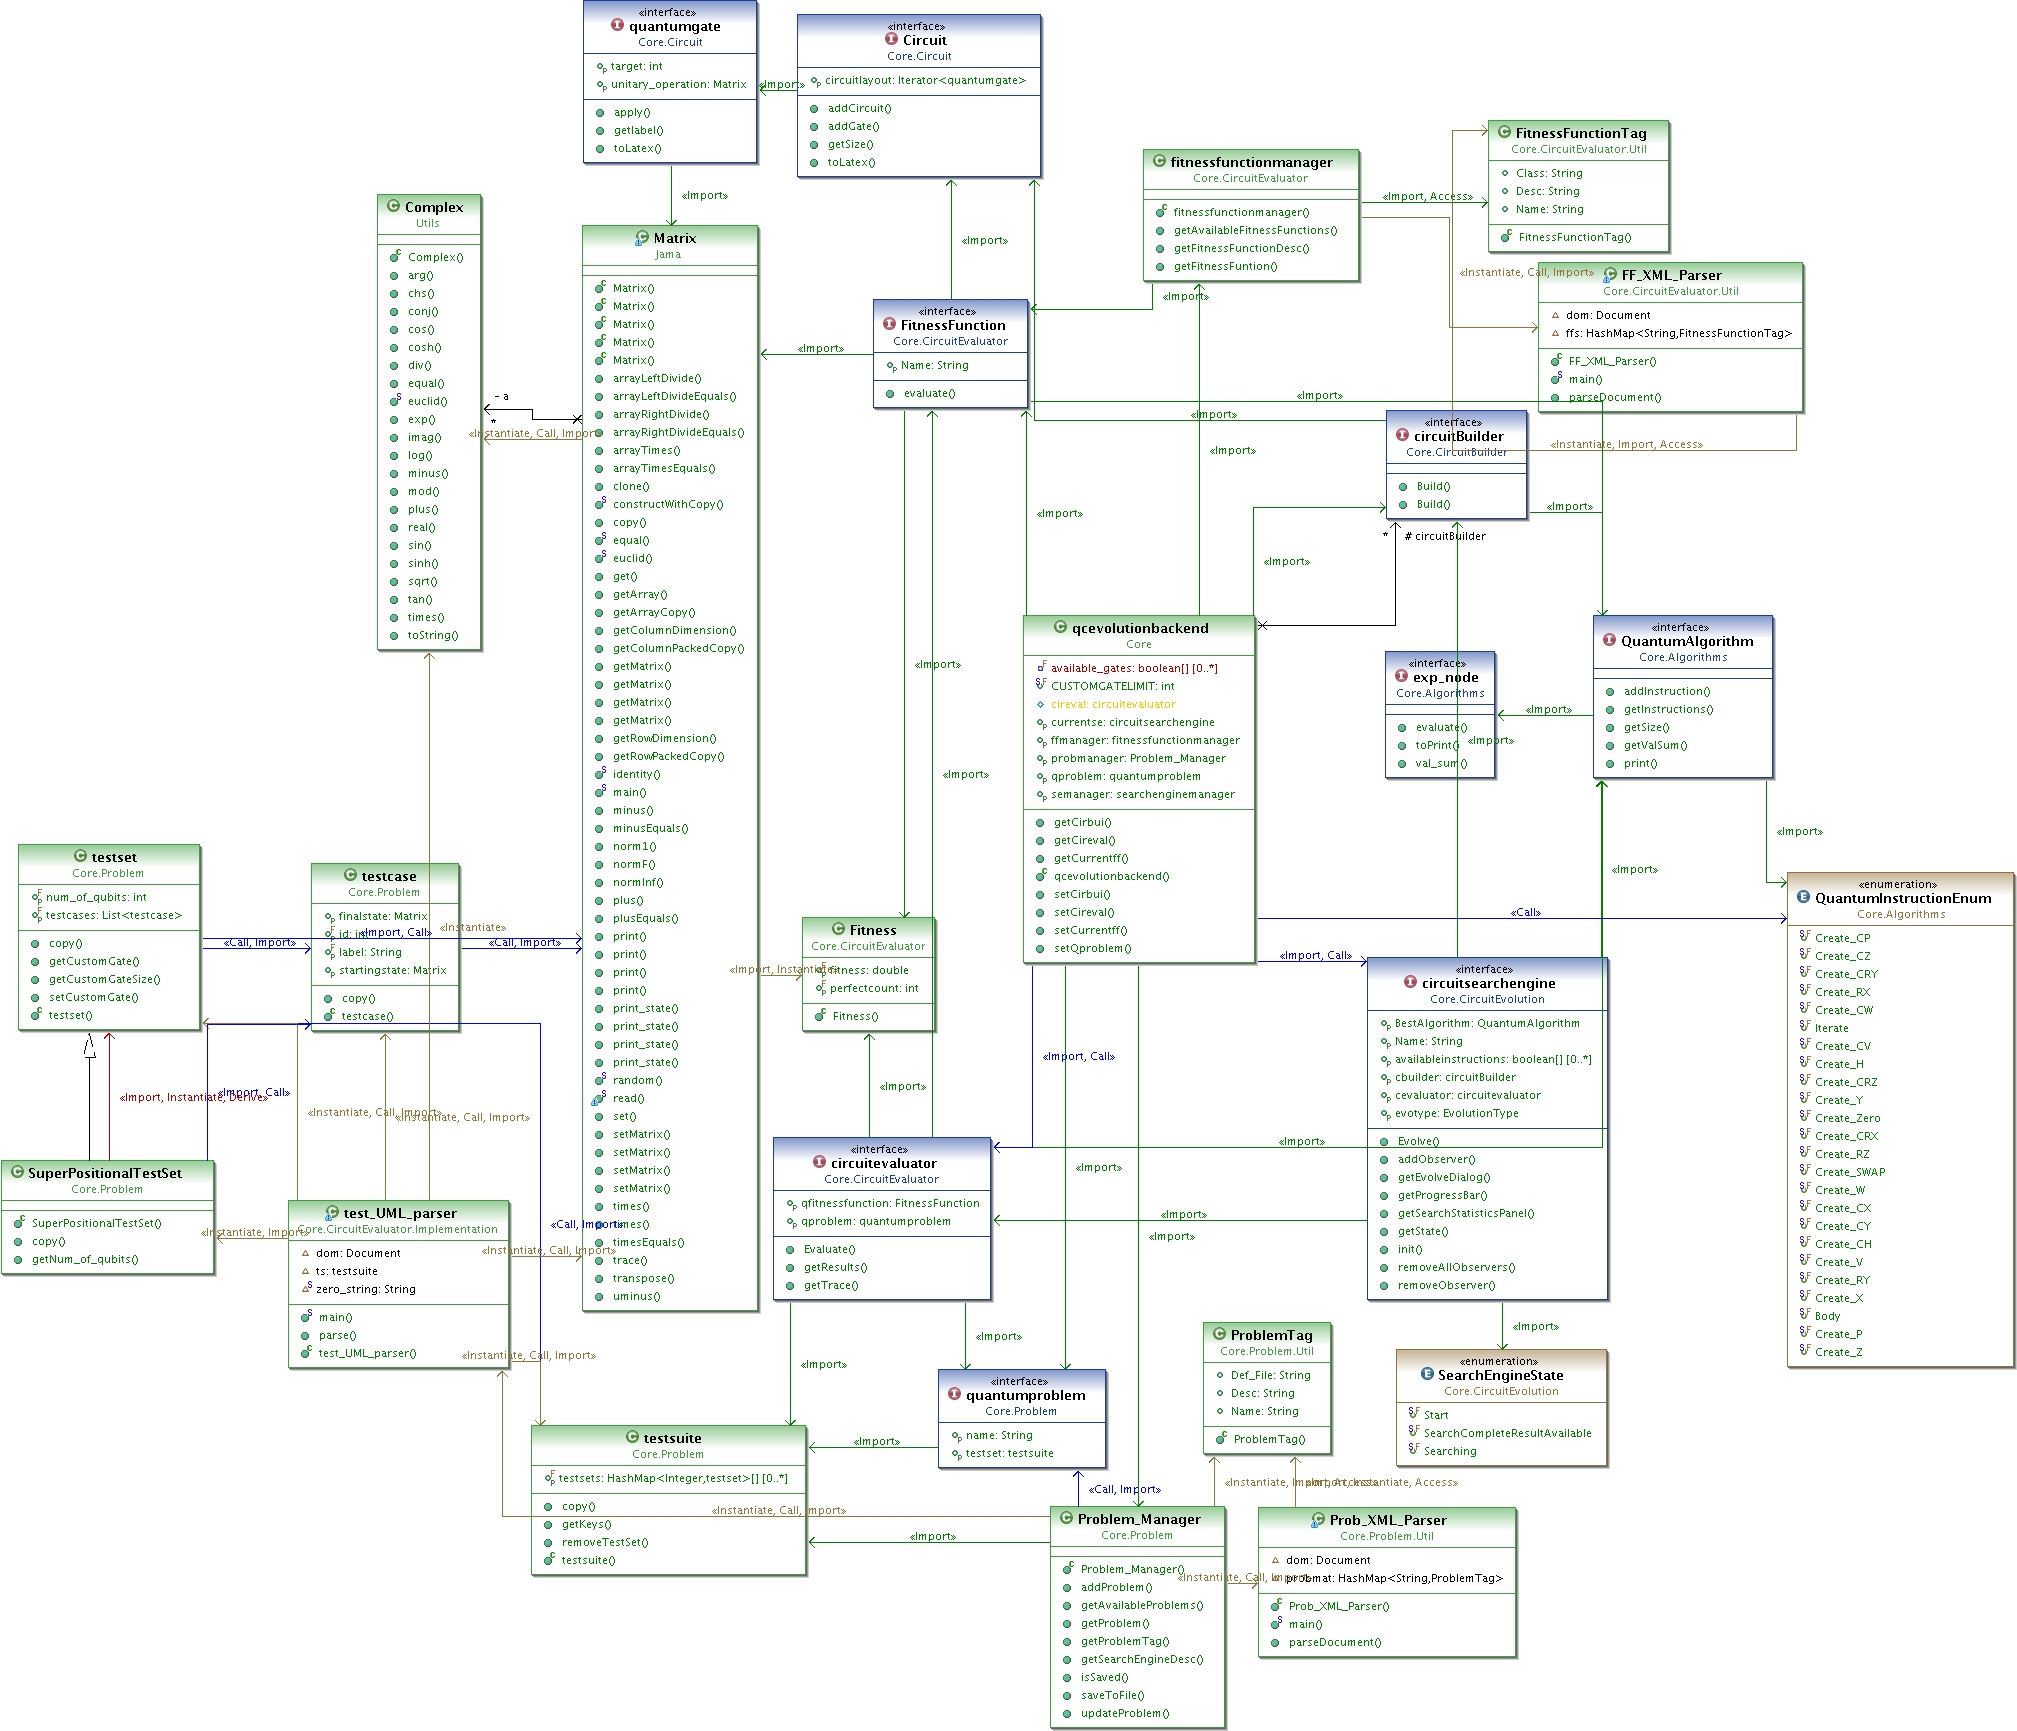
\includegraphics[height=0.85\textheight]{highlevelarchitecture.jpg}
\cleardoublepage
\endgroup

\chapter{XML Outlines}
\section{Search Engine XML Outline}
\label{sec:semanspecxml}
\lstset{language = XML}
\begin{lstlisting}
 <searchengine>
	<se>
	  <Name>SEARCH ENGINE NAMES</Name>
	  <Class>IMPLEMENTING FULLY QUALIFIED CLASS NAME</Class>
	  <Desc>SEARCH ENGINE DESCRIPTION</Desc>
	</se>
</searchengine>
\end{lstlisting}

\section{Problem Definition XML Outline}
\label{sec:probmanspecxml}
\lstset{language = XML}
\begin{lstlisting}
<Problems>
	<prob>
	  <Name>PROBLEM NAME</Name>
	  <DefFile>PROBLEM DEFINITION FILE</DefFile>
	  <Desc>PROBLEM DESCRIPTION</Desc>
	</prob>
</Problems>
\end{lstlisting}

\cleardoublepage
\begin{landscape}

\chapter{Available Algorithm Instructions}
\label{sec:alginstructionlist}
\centering
\begin{tabular}{|c|c|c|c|c|}
\hline
\textbf{Instruction} & \textbf{Action} & & \textbf{Instruction} & \textbf{Action}  \\
\hline
\textbf{Create\_H} & Create a Hadamard Gate & & \textbf{Create\_CH} & Create a Controlled Hadamard Gate \\
\hline
\textbf{Create\_X} & Create a Pauli-X Gate & & \textbf{Create\_CX} & Create a Controlled Pauli-X Gate \\
\hline
\textbf{Create\_Y} & Create a Pauli-Y Gate & & \textbf{Create\_CY} & Create a Controlled Pauli-Y Gate \\
\hline
\textbf{Create\_Z} & Create a Pauli-Z Gate & & \textbf{Create\_CZ} & Create a Controlled Pauli-Z Gate \\
\hline
\textbf{Create\_P} & Create a Phase Gate & & \textbf{Create\_CP} & Create a Controlled Phase Gate \\
\hline
\textbf{Create\_V} & Create a V Gate & & \textbf{Create\_CV} & Create a Controlled V Gate \\
\hline
\textbf{Create\_W} & Create a W Gate & & \textbf{Create\_CW} & Create a Controlled W Gate \\
\hline
\textbf{Create\_RX} & Create a Rotate-X Gate & & \textbf{Create\_CRX} & Create a Controlled Rotate-X Gate \\
\hline
\textbf{Create\_RY} & Create a Rotate-Y Gate & & \textbf{Create\_CRY} & Create a Controlled Rotate-Y Gate \\
\hline
\textbf{Create\_RZ} & Create a Rotate-Z Gate & & \textbf{Create\_CRZ} & Create a Controlled Rotate-Z Gate \\
\hline
\textbf{Create\_SWAP} & Create a SWAP Gate & &  &  \\
\hline
\textbf{Iterate} & Run Sub-Algorithm$[0]$ for $n$ iterations & & \textbf{RevIterate} & Run Sub-Algorithm$[0]$ for $n$ iterations in reverse order\\
\hline
\textbf{Body} & Perform each Sub-Algorithm in turn & & & \\
\hline
\textbf{Create\_Custom1} & Create Custom Gate Number $1$ & & \textbf{Create\_CCustom1} & Create a Controlled Custom Gate Number $1$ \\
\hline
\textbf{Create\_Custom2} & Create Custom Gate Number $2$ & & \textbf{Create\_CCustom2} & Create a Controlled Custom Gate Number $2$ \\
\hline
\textbf{Create\_Custom3} & Create Custom Gate Number $3$ & & \textbf{Create\_CCustom3} & Create a Controlled Custom Gate Number $3$ \\
\hline
\end{tabular}
\cleardoublepage
\end{landscape}